
\documentclass[border=8pt, multi, tikz]{standalone} 
\usepackage{import}
\subimport{../layers/}{init}
\usetikzlibrary{positioning}
\usetikzlibrary{3d} %for including external image 

\def\ConvColor{rgb:yellow,5;red,2.5;white,5}
\def\ConvReluColor{rgb:yellow,5;red,5;white,5}
\def\PoolColor{rgb:red,1;black,0.3}
\def\UnpoolColor{rgb:blue,2;green,1;black,0.3}
\def\FcColor{rgb:blue,5;red,2.5;white,5}
\def\FcReluColor{rgb:blue,5;red,5;white,4}
\def\SoftmaxColor{rgb:magenta,5;black,7}   
\def\SumColor{rgb:blue,5;green,15}
\def\BatchNormColor{rgb:blue,2;green, 3; yellow, 1}
\def\AvgPoolingColor{rgb:blue, 3; green,1}
\def\AddColor{rgb:blue, 255;green,255;red,255}

\newcommand{\copymidarrow}{\tikz \draw[-Stealth,line width=0.8mm,draw={rgb:blue,4;red,1;green,1;black,3}] (-0.3,0) -- ++(0.3,0);}

\begin{document}
\begin{tikzpicture}
\tikzstyle{connection}=[ultra thick,every node/.style={sloped,allow upside down},draw=\edgecolor,opacity=0.7]
\tikzstyle{copyconnection}=[ultra thick,every node/.style={sloped,allow upside down},draw={rgb:blue,4;red,1;green,1;black,3},opacity=0.7]

\node[canvas is zy plane at x=0] (temp) at (-3,0,0) {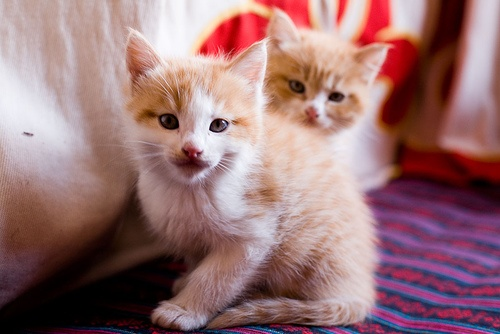
\includegraphics[width=8cm,height=8cm]{../examples/fcn8s/cats.jpg}};

\pic[shift={(1, 0, 0)}] at (0,0,0) 
    {Box={
        name=conv1,
        caption= ,
        xlabel={{224, }},
        zlabel={32x3},
        fill=\ConvColor,
        height=40,
        width=4,
        depth=45
        }
    };

\pic[shift={(1.5, 0, 0)}] at (0,0,0) 
    {RightBandedBox={
        name=batch_norm,
        caption= ,
        xlabel={{112, }},
        zlabel={32x64},
        fill=\BatchNormColor,
        bandfill=\FcReluColor,
        height=40,
        width=2,
        depth=45
        }
    };


\pic[shift={ (2.5, 0, 0) }] at (0,0,0) 
    {Box={
        name=maxpooling,
        caption= ,
        fill=\PoolColor,
        opacity=0.5,
        height=40,
        width=2,
        depth=45
        }
    };

\pic[shift={(5, 0, 0)}] at (0,0,0) 
    {Box={
        name=conv1x1,
        caption= ,
        xlabel={{56, }},
        zlabel={32x64},
        fill=\ConvColor,
        height=20,
        width=4,
        depth=25
        }
    };

\pic[shift={(5.5, 0, 0)}] at (0,0,0) 
    {RightBandedBox={
        name=batch_norm2,
        caption= ,
        xlabel={{56, }},
        zlabel={32x256},
        fill=\BatchNormColor,
        bandfill=\FcReluColor,
        height=20,
        width=2,
        depth=25
        }
    };

\pic[shift={(7, 0, 0)}] at (0,0,0) 
    {Box={
        name=conv3x3,
        caption= ,
        xlabel={{56, }},
        zlabel={32x256},
        fill=\ConvColor,
        height=20,
        width=4,
        depth=25
        }
    };

\pic[shift={(7.5, 0, 0)}] at (0,0,0) 
    {RightBandedBox={
        name=batch_norm3,
        caption= ,
        xlabel={{56, }},
        zlabel={32x256},
        fill=\BatchNormColor,
        bandfill=\FcReluColor,
        height=20,
        width=2,
        depth=25
        }
    };

\pic[shift={(10, 0, 0)}] at (0,0,0) 
    {Box={
        name=conv1x1_2,
        caption= ,
        xlabel={{56, }},
        zlabel={32x256},
        fill=\ConvColor,
        height=20,
        width=4,
        depth=25
        }
    };

\pic[shift={(10.5, 0, 0)}] at (0,0,0) 
    {RightBandedBox={
        name=batch_norm4,
        caption= ,
        xlabel={{56, }},
        zlabel={32x256},
        fill=\BatchNormColor,
        bandfill=\AddColor,
        height=20,
        width=2,
        depth=25
        }
    };

\pic[shift={(12.5, 0, 0)}] at (0,0,0) 
    {Box={
        name=add2,
        caption= ,
        xlabel={{56, }},
        zlabel={32x256},
        fill=\AddColor,
        height=20,
        width=4,
        depth=25
        }
    };

\pic[shift={(18, 0, 0)}] at (0,0,0) 
    {Box={
        name=relu4,
        caption= ,
        xlabel={{56, }},
        zlabel={32x256},
        fill=\FcReluColor,
        height=20,
        width=4,
        depth=25
        }
    };

\pic[shift={(21, 0, 0)}] at (0,0,0) 
    {Box={
        name=glavgpooling,
        caption= ,
        xlabel={{56, }},
        zlabel={32x256},
        fill=\AvgPoolingColor,
        height=20,
        width=4,
        depth=25
        }
    };

\pic[shift={(23, 0, 0)}] at (0,0,0) 
    {Box={
        name=flatten,
        caption= ,
        xlabel={{56, }},
        zlabel={32x256},
        fill=\ConvColor,
        height=40,
        width=4,
        depth=25
        }
    };

\pic[shift={(25, 0, 0)}] at (0,0,0) 
    {Box={
        name=fc,
        caption= ,
        xlabel={{56, }},
        zlabel={32x256},
        fill=\ConvColor,
        height=40,
        width=4,
        depth=25
        }
    };

\draw [connection]  (maxpooling-east)    -- node {\midarrow} (conv1x1-west);

\draw [connection]  (batch_norm2-east)    -- node {\midarrow} (conv3x3-west);

\draw [connection]  (batch_norm3-east)    -- node {\midarrow} (conv1x1_2-west);

\draw [connection]  (batch_norm4-east)    -- node {\midarrow} (add2-west);

\draw [connection]  (add2-east)    -- node {\midarrow} (relu4-west);

\draw [connection]  (relu4-east)    -- node {\midarrow} (glavgpooling-west);

\draw [connection]  (glavgpooling-east)    -- node {\midarrow} (flatten-west);

\draw [connection]  (flatten-east)    -- node {\midarrow} (fc-west);


\node (33 Iterations) at (12.5, 10, 0) {33 Iterations};

\draw[connection, to path={-| (\tikztotarget)}]
  (add2-east) edge (33 Iterations) (33 Iterations) edge (conv1x1-west);


\end{tikzpicture}
\end{document}
